\documentclass[serif,mathserif]{beamer}
\usepackage{amsmath, amsfonts, epsfig, xspace}
%\usepackage{algorithm,algorithmic}
%\usepackage{pstricks,pst-node}
\usepackage{multimedia}
\usepackage[normal,tight,center]{subfigure}
\setlength{\subfigcapskip}{-.5em}
\usepackage{beamerthemesplit}
\usetheme{lankton-keynote}

\author[Tejaswi KC, Raj Krishnan]{Group 11 \\ Tejaswi KC \quad Raj Krishnan \\ 140010020 \quad 140010007}

\title[PyAlpha\hspace{2em}\insertframenumber/\inserttotalframenumber]{PyAlpha: Final Report}

\institute{Indian Institute of Technology, Bombay}

\begin{document}

    \maketitle

    \begin{frame}

        \frametitle{Tasks}

        \begin{itemize}
            \item Build a python module to handle the purchase and sale of stocks
                  as per current prices on the share markets
            \item Build a module to compute the quality of various alphas
                  (weights for various stocks)
        \end{itemize}

    \end{frame}

    \begin{frame}

        \frametitle{Source Code}

        \begin{itemize}
            \item Hosted at \url{https://github.com/raj-krishnan/PyAlpha}
            \item Documentation hosted at \url{pyalpha.readthedocs.io/}
            \item Continuous Integration using \href{https://travis-ci.org/raj-krishnan/PyAlpha}{Travis}
            \item Coverage Testing using \href{https://coveralls.io/github/raj-krishnan/PyAlpha}{Coveralls}
        \end{itemize}

    \end{frame}

    \begin{frame}

        \frametitle{Dependencies}

        \begin{itemize}
            \item pandas
            \item peewee
            \item ystockquote
            \item numpy
        \end{itemize}

    \end{frame}

    \begin{frame}

        \frametitle{Installation}

        \begin{itemize}
            \item git clone https://github.com/raj-krishnan/PyAlpha.git
            \item cd PyAlpha
            \item pip install -r requirements.txt
            \item python setup.py install
            \item nosetests
        \end{itemize}

    \end{frame}

    % \begin{frame}

    %     \frametitle{Demo}

    %     \begin{figure}[h]
    %         \centering
    %         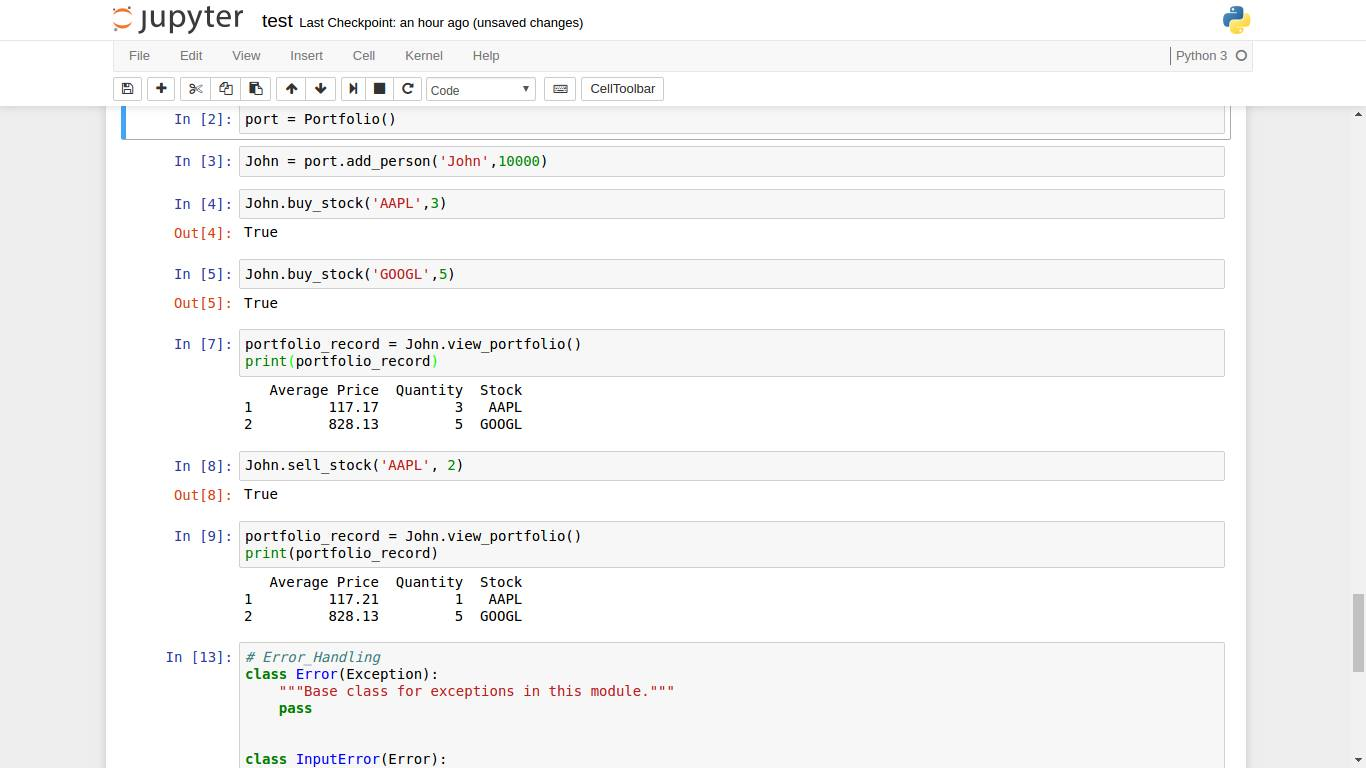
\includegraphics[width=\linewidth]{demo.png}
    %     \end{figure}

    % \end{frame}

    \begin{frame}
        \centering \huge{Questions}
    \end{frame}

    \begin{frame}
        \centering \huge{Thank You!}
    \end{frame}

\end{document}
